% ══════════════════════════════════════════════════════════════════════════
% ReBeL in this codebase — from the idea to the code (trainer/rebel_py)
% Companion to modern_poker_ai_tutorial.pdf (its ReBeL section is the "theory"
% side; this document maps that theory onto the implementation).
% Build:  pdflatex rebel_implementation.tex   (run twice for refs/toc)
% ══════════════════════════════════════════════════════════════════════════
\documentclass[11pt,a4paper]{article}

\usepackage[utf8]{inputenc}
\usepackage[T1]{fontenc}
\usepackage{lmodern}
\usepackage[margin=2.2cm]{geometry}
\usepackage{amsmath,amssymb}
\usepackage[dvipsnames]{xcolor}
\usepackage{tikz}
\usetikzlibrary{arrows.meta,positioning,shapes.geometric,calc,fit,backgrounds}
\usepackage{listings}
\usepackage{tcolorbox}
\usepackage{booktabs}
\usepackage{enumitem}
\usepackage[colorlinks=true,linkcolor=MidnightBlue,urlcolor=MidnightBlue,citecolor=MidnightBlue]{hyperref}

% ─── Palette (same as the tutorials) ────────────────────────────────────────
\definecolor{accent}{RGB}{25,55,110}
\definecolor{heroG}{RGB}{20,110,60}
\definecolor{villR}{RGB}{160,40,40}
\definecolor{memO}{RGB}{190,110,10}
\definecolor{codebg}{RGB}{246,247,249}
\definecolor{codekw}{RGB}{0,80,160}
\definecolor{codecomment}{RGB}{100,120,100}
\definecolor{codestr}{RGB}{150,60,20}

\lstdefinestyle{py}{
  language=Python,
  basicstyle=\ttfamily\small,
  keywordstyle=\color{codekw}\bfseries,
  commentstyle=\color{codecomment}\itshape,
  stringstyle=\color{codestr},
  backgroundcolor=\color{codebg},
  frame=single, rulecolor=\color{black!25},
  framesep=6pt, xleftmargin=10pt, xrightmargin=4pt,
  showstringspaces=false,
  columns=fullflexible, keepspaces=true,
  breaklines=true,
  literate={σ}{$\sigma$}1 {β}{$\beta$}1 {θ}{$\theta$}1 {≈}{$\approx$}1
           {×}{$\times$}1 {→}{$\rightarrow$}1 {Σ}{$\Sigma$}1 {·}{$\cdot$}1
}

\newtcolorbox{intuition}{
  colback=blue!4, colframe=accent, boxrule=0.8pt, arc=2mm,
  title=\textbf{Intuition}, fonttitle=\color{white},
  left=6pt, right=6pt, top=4pt, bottom=4pt}
\newtcolorbox{trap}{
  colback=red!4, colframe=villR, boxrule=0.8pt, arc=2mm,
  title=\textbf{Watch out}, fonttitle=\color{white},
  left=6pt, right=6pt, top=4pt, bottom=4pt}
\newtcolorbox{defbox}{
  colback=black!3, colframe=black!50, boxrule=0.6pt, arc=2mm,
  left=6pt, right=6pt, top=4pt, bottom=4pt}

\setlength{\parskip}{4pt}
\setlength{\parindent}{0pt}
\newcommand{\file}[1]{\textcolor{accent}{\texttt{#1}}}
\newcommand{\fn}[1]{\texttt{#1}}

\begin{document}

% ─── Title ──────────────────────────────────────────────────────────────────
\begin{center}
  {\Huge\bfseries ReBeL, in this codebase}\\[2mm]
  {\large from the idea to the code --- a guided tour of \texttt{trainer/rebel\_py}}\\[3mm]
  {\normalsize Combining Deep RL and Search on public belief states, implemented for
   heads-up no-limit hold'em}\\[2mm]
  {\small Companion to \texttt{docs/modern\_poker\_ai\_tutorial.pdf} --- that document
   is the \emph{theory}; this one is the \emph{map from theory to code}.}
\end{center}
\vspace{2mm}
\hrule
\vspace{3mm}

\begin{intuition}
ReBeL's one idea (tutorial, §ReBeL): an imperfect-information game becomes a
\emph{perfect-information} game if the state is the \textbf{public belief state}
(PBS). Then AlphaZero-style self-play $+$ search applies, with \textbf{CFR}
doing the searching and a \textbf{value net $V(\text{PBS})$} pricing the leaves of
depth-limited subgames. This codebase is a paper-faithful, from-scratch
implementation of that idea over the project's poker engine. Every ReBeL concept
below is named with the file and function that realizes it.
\end{intuition}

\tableofcontents
\vspace{3mm}\hrule

% ════════════════════════════════════════════════════════════════════════════
\section{High-level view: the module map}
% ════════════════════════════════════════════════════════════════════════════

The package \file{trainer/rebel\_py/} is pure Python, vectorized over the
\textbf{1326} hole-card combinations with NumPy, and reuses the project's pybind
engine (\texttt{pokertrainer\_engine}) only to enumerate legal bets and evaluate
7-card hands. It is built in layers: ground-truth game machinery at the bottom,
the value-net self-play loop in the middle, the cluster trainer on top. The
layers were validated bottom-up (each has a hard correctness gate before the
one above it was written).

\begin{center}
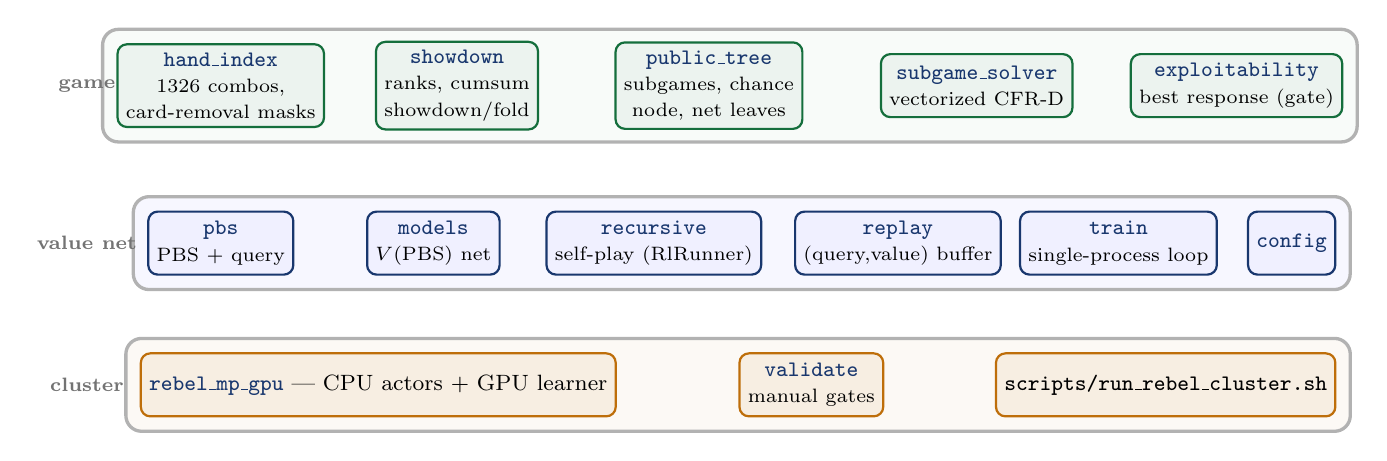
\begin{tikzpicture}[font=\footnotesize, >={Stealth[length=2mm]},
  box/.style={rectangle, rounded corners=1.2mm, draw, thick, align=center,
              minimum height=8mm, inner sep=3pt, fill=white},
  lay/.style={rectangle, rounded corners=2mm, draw=black!30, very thick,
              inner sep=5pt},
  lbl/.style={font=\scriptsize\bfseries, text=black!55}]

% Layer 1: game machinery
\node[box, fill=heroG!8, draw=heroG] (hi)  at (0,0)   {\file{hand\_index}\\ \scriptsize 1326 combos,\\ \scriptsize card-removal masks};
\node[box, fill=heroG!8, draw=heroG] (sd)  at (3.0,0) {\file{showdown}\\ \scriptsize ranks, cumsum\\ \scriptsize showdown/fold};
\node[box, fill=heroG!8, draw=heroG] (pt)  at (6.2,0) {\file{public\_tree}\\ \scriptsize subgames, chance\\ \scriptsize node, net leaves};
\node[box, fill=heroG!8, draw=heroG] (ss)  at (9.6,0) {\file{subgame\_solver}\\ \scriptsize vectorized CFR-D};
\node[box, fill=heroG!8, draw=heroG] (ex)  at (12.9,0){\file{exploitability}\\ \scriptsize best response (gate)};
\node[lbl] at (-1.7,0) {game};

% Layer 2: value-net loop
\node[box, fill=blue!6, draw=accent] (pbs) at (0,-2.0)  {\file{pbs}\\ \scriptsize PBS + query};
\node[box, fill=blue!6, draw=accent] (mo)  at (2.7,-2.0){\file{models}\\ \scriptsize $V(\text{PBS})$ net};
\node[box, fill=blue!6, draw=accent] (re)  at (5.5,-2.0){\file{recursive}\\ \scriptsize self-play (RlRunner)};
\node[box, fill=blue!6, draw=accent] (rp)  at (8.6,-2.0){\file{replay}\\ \scriptsize (query,value) buffer};
\node[box, fill=blue!6, draw=accent] (tr)  at (11.4,-2.0){\file{train}\\ \scriptsize single-process loop};
\node[box, fill=blue!6, draw=accent] (cf)  at (13.6,-2.0){\file{config}};
\node[lbl] at (-1.7,-2.0) {value net};

% Layer 3: cluster
\node[box, fill=memO!12, draw=memO, minimum width=42mm] (mp) at (2.0,-3.8)
     {\file{rebel\_mp\_gpu} --- CPU actors + GPU learner};
\node[box, fill=memO!12, draw=memO] (vl) at (7.5,-3.8) {\file{validate}\\ \scriptsize manual gates};
\node[box, fill=memO!12, draw=memO, minimum width=42mm] (sc) at (12.0,-3.8)
     {\texttt{scripts/run\_rebel\_cluster.sh}};
\node[lbl] at (-1.7,-3.8) {cluster};

\begin{scope}[on background layer]
  \node[lay, fit=(hi)(ex), fill=heroG!3] {};
  \node[lay, fit=(pbs)(cf), fill=blue!3] {};
  \node[lay, fit=(mp)(sc), fill=memO!4] {};
\end{scope}
\end{tikzpicture}
\end{center}

\paragraph{The phases (how it was built and validated).}
\begin{center}\small
\begin{tabular}{@{}llll@{}}
\toprule
Phase & What & Gate (proof it is correct) & Commit \\
\midrule
1   & CFR-D solver, \emph{no} net          & push/fold $=$ Nash oracle; river $\to 0$ exploit. & \texttt{7b3d718} \\
2a  & value net, river depth limit         & self-play drops exploit. $2.0\to0.04$ bb/hand     & \texttt{a353fc7} \\
2b  & river \textbf{chance node} (turn$\to$river) & ground truth $\to 0.027$; equity $=$ \texttt{evaluate7} & \texttt{030b282}, \texttt{afe6928} \\
3   & cluster trainer (actors $+$ learner) & river $1.1\to0.9$; checkpoints, TorchScript       & \texttt{8425c52} \\
--  & scaling (rank/incidence leaves)      & exact vs dense; $1.7$\,GB$\to5$\,MB, $110\to11$\,s & \texttt{83e1a75}, \texttt{9e7217b} \\
\bottomrule
\end{tabular}
\end{center}

% ════════════════════════════════════════════════════════════════════════════
\section{The conversion trick in code: PBS and the query (\file{pbs.py})}
% ════════════════════════════════════════════════════════════════════════════

\begin{defbox}
\textbf{Public belief state.} Everything public (board, street, pot, who acts,
amount to call, stack) \emph{plus} both players' belief vectors over the 1326
hole combos. In code the public part is \fn{PublicState} (a dataclass); the
beliefs are two \texttt{np.ndarray} of length 1326 carried alongside.
\end{defbox}

The value net cannot eat a Python object; \fn{encode\_query} flattens a PBS (as
seen by a chosen \emph{traverser}) into the fixed float vector the net consumes.
It mirrors \texttt{write\_query\_to} in the reference Liar's Dice C++ code, but
with poker's richer public state:

\begin{lstlisting}[style=py, caption={\file{pbs.py} --- the PBS$\to$vector encoding. Two faithfulness points: beliefs are normalized to sum 1 (so the net learns value \emph{per unit opponent mass}), with the same $10^{-80}$ smoothing so an all-zero reach maps to uniform, not NaN.}]
def encode_query(traverser, ps, reach0, reach1):
    q = np.empty(query_dim())                  # 2710 floats
    q[0] = ps.to_act                           # who acts (0=SB / 1=BB)
    q[1] = traverser                           # whose value the net should output
    q[2] = ps.street / 3.0                     # 0..3 (one net spans streets)
    q[3] = ps.pot_bb / POT_SCALE               # scalars normalized into [0,1]-ish
    q[4] = ps.to_call_bb / POT_SCALE
    q[5] = ps.stack_bb / POT_SCALE
    q[6:6+52]        = board_multi_hot(ps.board)        # which cards are out
    q[58:58+1326]    = normalize_safe(reach0)           # player-0 beliefs
    q[58+1326:]      = normalize_safe(reach1)           # player-1 beliefs
    return q                                            # dim = 6 + 52 + 2*1326
\end{lstlisting}

\begin{center}\small
\begin{tabular}{@{}llr@{}}
\toprule
slice & meaning & width \\
\midrule
\texttt{q[0:6]}    & \texttt{to\_act, traverser, street, pot, to\_call, stack} & 6 \\
\texttt{q[6:58]}   & board multi-hot (52 cards)                                & 52 \\
\texttt{q[58:1384]}& player-0 belief (normalized)                              & 1326 \\
\texttt{q[1384:2710]}& player-1 belief (normalized)                            & 1326 \\
\midrule
& \textbf{total \fn{query\_dim()}} & \textbf{2710} \\
\bottomrule
\end{tabular}
\end{center}

\begin{intuition}
Why feed \emph{both} players' beliefs and a \texttt{traverser} flag, rather than
``my beliefs / your beliefs''? Because the subgame's value depends on the whole
PBS, and ReBeL computes \emph{all} beliefs (tutorial, Q ``how does ReBeL know the
opponent's beliefs?''): it never observes them, it \emph{computes} them by Bayes
from common-knowledge strategies. The \texttt{traverser} bit just selects which
player's per-hand values the net should return for this query.
\end{intuition}

% ════════════════════════════════════════════════════════════════════════════
\section{The depth-limited subgame (\file{public\_tree.py})}
% ════════════════════════════════════════════════════════════════════════════

Tutorial step (2) is ``build the depth-limited subgame --- shape only, no leaf
values yet''. That is exactly \fn{build\_river\_subgame} / \fn{build\_turn\_subgame}:
they walk the engine to a public state, then enumerate the betting tree by
cloning and stepping \texttt{Env}. A \fn{Node} is a \emph{public} state (betting
sequence) --- hole-independent, so one tree serves all 1326 hands. Leaves are of
three kinds:

\begin{center}
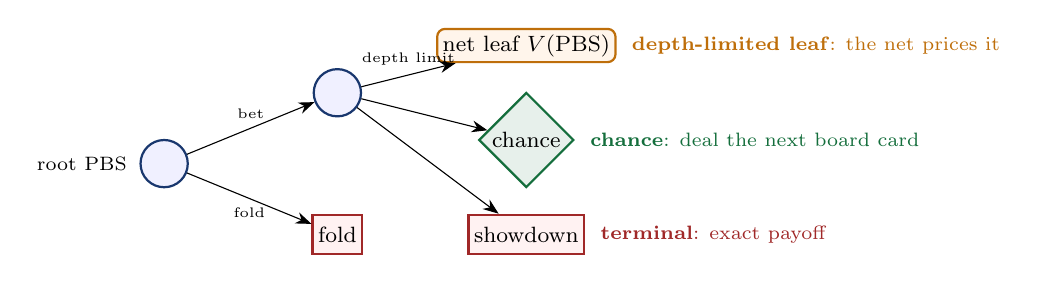
\begin{tikzpicture}[font=\footnotesize, >={Stealth[length=2mm]},
  d/.style={circle, draw=accent, fill=blue!6, thick, minimum size=6mm, inner sep=0},
  t/.style={rectangle, draw=villR, fill=red!5, thick, minimum size=5mm, inner sep=2pt},
  n/.style={rectangle, rounded corners=1mm, draw=memO, fill=orange!8, thick, inner sep=2pt},
  c/.style={diamond, draw=heroG, fill=heroG!10, thick, inner sep=1pt}]
  \node[d] (r) at (0,0) {};
  \node[font=\scriptsize, left=1pt of r] {root PBS};
  \node[d] (a) at (2.2,0.9) {};
  \node[t] (f) at (2.2,-0.9) {fold};
  \node[n] (nl) at (4.6,1.5) {net leaf $V(\text{PBS})$};
  \node[c] (ch) at (4.6,0.3) {chance};
  \node[t] (sd) at (4.6,-0.9) {showdown};
  \draw[->] (r) -- node[above,font=\tiny]{bet} (a);
  \draw[->] (r) -- node[below,font=\tiny]{fold} (f);
  \draw[->] (a) -- node[above,font=\tiny]{depth limit} (nl);
  \draw[->] (a) -- (ch);
  \draw[->] (a) -- (sd);
  \node[font=\scriptsize, right=2pt of nl, align=left, text=memO]
    {\textbf{depth-limited leaf}: the net prices it};
  \node[font=\scriptsize, right=2pt of ch, align=left, text=heroG]
    {\textbf{chance}: deal the next board card};
  \node[font=\scriptsize, right=2pt of sd, align=left, text=villR]
    {\textbf{terminal}: exact payoff};
\end{tikzpicture}
\end{center}

\textbf{Terminal value closures.} Each leaf stores a closure
\texttt{term\_value(traverser, opp\_reach)$\to$(1326,)} that returns the per-hand
counterfactual value against the opponent's \emph{reach} (so card removal is
folded into the reach). Showdown and fold are derived in §\ref{sec:scale} without
any $1326^2$ matrix.

\textbf{Net leaves} are how the depth limit is realized: a non-terminal node at
the limit becomes \texttt{is\_net\_leaf=True} and carries its \fn{PublicState}, so
the solver can build the query and ask the net. The depth limit follows the
paper: \emph{stop where new cards would be dealt}.

\textbf{The chance node} (Phase 2b) is the river card. The engine pre-deals all
five board cards, so at the turn the active board is the first four and the river
ranges over the 48 unseen cards. The betting \emph{shape} is board-independent,
so one river subtree is re-parametrized per card by its showdown. Card removal is
handled exactly (next section).

\begin{lstlisting}[style=py, caption={\file{public\_tree.py} --- re-rooting/truncating an already-built tree. This is how the ReBeL recursion ``builds a fresh subgame at each public state'' without touching the engine: \fn{subtree\_subgame} copies the subtree from any node and turns chance children (or depth-limit nodes) into value-net leaves.}]
def subtree_subgame(full, root_nid, max_depth, stop_at_chance=False):
    # decision nodes at max_depth -> net leaves (carry their PublicState);
    # with stop_at_chance, a chance node's children become river-PBS net leaves
    # -> this is the ReBeL "turn subgame": solve turn betting, net values the river.
    ...
\end{lstlisting}

% ════════════════════════════════════════════════════════════════════════════
\section{The search engine: vectorized CFR-D (\file{subgame\_solver.py})}
% ════════════════════════════════════════════════════════════════════════════

Tutorial step (3): ``$T_{\mathrm{cfr}}$ iterations of tabular CFR inside $G_t$,
with leaf evaluation \emph{inside every iteration} --- strategy and leaf values
co-evolve.'' \fn{CfrSolver} is a faithful, vectorized port of the reference
\texttt{CFR} in \texttt{subgame\_solving.cc}: every per-node quantity is a
\texttt{(1326, n\_actions)} or \texttt{(1326,)} array, so all 1326 hands are
updated at once. One \fn{step(traverser)} does:

\begin{enumerate}[leftmargin=1.6em, itemsep=0pt]
\item compute both players' reaches top-down under the current strategy;
\item \textbf{price the net leaves} (the co-evolution): query $V$ at every net
  leaf with the \emph{current} normalized reaches, scale by opponent reach mass;
\item back values up (accumulate regret at traverser nodes, sum at opponent
  nodes, $\tfrac{1}{44}$-average at chance nodes);
\item regret-matching $\to$ new current strategy; reach-weight it into the
  running average ($=\bar\sigma$, the converging object).
\end{enumerate}

\begin{lstlisting}[style=py, caption={\file{subgame\_solver.py} --- the leaf-value scaling trick, the single most important detail. The net outputs values assuming the opponent belief is normalized to sum 1; the solver recovers the true counterfactual leaf value by multiplying by the opponent's reach \emph{mass} at that leaf. This decoupling lets one net generalize across subgames with wildly different reach magnitudes.}]
def _compute_net_leaf_values(self, traverser):
    opp = 1 - traverser
    queries = np.stack([encode_query(traverser, nd.public_state,
                                     self.reach[0][nid], self.reach[1][nid])
                        for nid in self.net_leaves])          # normalized inside
    vals = self.value_fn(queries)                             # (N, 1326), normalized
    for row, nid in enumerate(self.net_leaves):
        mass = self.reach[opp][nid].sum()                     # opponent reach MASS
        self.values[nid] = vals[row] * self.net_leaf_valid[nid] * mass
\end{lstlisting}

\begin{trap}
The training target uses the \emph{same} convention. \fn{get\_hand\_values}
returns \texttt{root\_values\_means} --- the linear-CFR running mean of the root
counterfactual values --- computed with the root beliefs normalized to sum 1
(mass $=1$). So ``net output $\times$ opponent mass'' at a leaf and ``root value
at mass 1'' as a label are consistent. Get this wrong and the net learns a
mis-scaled value function that silently caps how low exploitability can go.
\end{trap}

\textbf{The chance node} couples turn and river inside one CFR. Reaching down, it
masks each player's reach by the dealt card; backing up, it averages the 48 river
values with the matchup normalizer $\tfrac{1}{44}$ (= $52-4$ board $-2$ hero $-2$
opp). Best response (\file{exploitability.py}) handles chance the same way; its
value at the root is the \emph{exploitability gate} used everywhere.

% ════════════════════════════════════════════════════════════════════════════
\section{The value network (\file{models.py})}
% ════════════════════════════════════════════════════════════════════════════

ReBeL's value net is the AlphaZero analogue: $V(\text{PBS})\to$ per-hand values.
We follow the reference \texttt{Net2} exactly --- a GELU MLP whose \textbf{output
layer is scaled by 0.01 at init} so the net's first predictions are near zero (a
near-zero value function is the safe starting point for the bootstrapping below).
One net spans all streets; the board and street live in the query.

\begin{center}
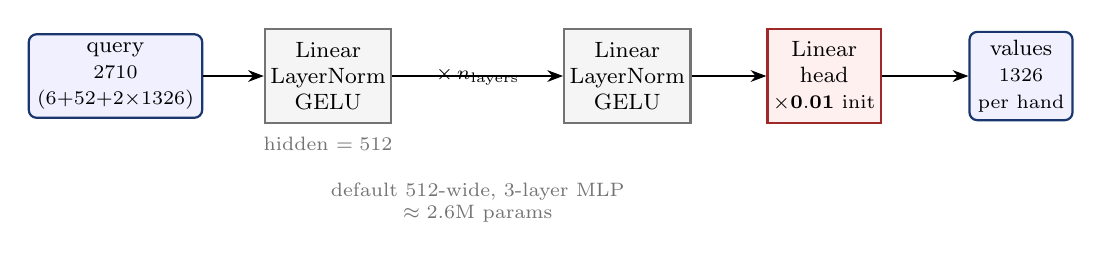
\begin{tikzpicture}[font=\footnotesize, >={Stealth[length=2mm]},
  io/.style={rectangle, rounded corners=1mm, draw=accent, fill=blue!6, thick,
             align=center, minimum height=9mm, inner sep=3pt},
  lyr/.style={rectangle, draw=black!55, fill=black!4, thick, align=center,
              minimum height=12mm, minimum width=15mm, inner sep=2pt},
  hd/.style={rectangle, draw=villR, fill=red!6, thick, align=center,
             minimum height=12mm, inner sep=2pt}]
  \node[io] (q) at (0,0) {query\\ \scriptsize 2710\\ \scriptsize (6+52+2$\times$1326)};
  \node[lyr] (l1) at (2.7,0) {Linear\\ LayerNorm\\ GELU};
  \node[font=\scriptsize] (rep) at (4.6,0) {$\times\,n_{\text{layers}}$};
  \node[lyr] (l2) at (6.5,0) {Linear\\ LayerNorm\\ GELU};
  \node[hd] (h) at (9.0,0) {Linear\\ head\\ \scriptsize $\mathbf{\times 0.01}$ init};
  \node[io] (o) at (11.5,0) {values\\ \scriptsize 1326\\ \scriptsize per hand};
  \draw[->] (q)--(l1); \draw[->] (l1)--(l2); \draw[->] (l2)--(h); \draw[->] (h)--(o);
  \node[font=\scriptsize, below=1pt of l1, text=black!55] {hidden $=512$};
  \node[font=\scriptsize, below=10mm of rep, align=center, text=black!55]
    {default $512$-wide, $3$-layer MLP\\ $\approx 2.6$M params};
\end{tikzpicture}
\end{center}

\begin{lstlisting}[style=py, caption={\file{models.py} --- the net and the numpy adapter the solver calls. \fn{NetValueFn} is the bridge: numpy queries in, numpy values out, eval/no-grad, on the net's device. Card-removal/opp-mass scaling is the solver's job (previous section).}]
class ValueNet(nn.Module):
    def __init__(self, query_dim, n_hidden=512, n_layers=3, out_size=1326):
        self.body = build_mlp(n_in=query_dim, n_hidden=n_hidden,
                              n_layers=n_layers, use_layer_norm=True)   # GELU
        self.head = nn.Linear(n_hidden, out_size)
        with torch.no_grad():
            self.head.weight *= 0.01; self.head.bias *= 0.01            # near-zero V

class NetValueFn:                       # queries (N,2710) -> values (N,1326)
    def __call__(self, queries):
        with torch.no_grad():
            return self.net(torch.as_tensor(queries, ...)).cpu().numpy()
\end{lstlisting}

\begin{intuition}
\textbf{What the net sees and says} (tutorial §``what the value net actually sees
and says''). \emph{Sees}: the PBS query --- public scalars, board, both belief
vectors. \emph{Says}: for the queried traverser, the value of \emph{each} of its
1326 hands at this PBS under near-equilibrium play. It is a \emph{range}-valued
function, which is why ReBeL ``solves for your whole range, not your hand'': the
solver needs values for every hand to run CFR, and one query returns all of them.
\end{intuition}

% ════════════════════════════════════════════════════════════════════════════
\section{The self-play loop (\file{recursive.py})}
% ════════════════════════════════════════════════════════════════════════════

\fn{RlRunner.step} is the tutorial's six-step episode (\texttt{rebel\_episode}),
one hand of self-play. The correspondence is line-for-line:

\begin{center}\small
\begin{tabular}{@{}p{0.40\textwidth}p{0.55\textwidth}@{}}
\toprule
tutorial step & \file{recursive.py} \\
\midrule
(1) freeze PBS $\beta_t$            & current \texttt{node\_id} $+$ \texttt{beliefs} \\
(2) build depth-limited subgame     & \fn{subtree\_subgame(full, node\_id, $\cdot$, stop\_at\_chance)} \\
(3) solve with CFR (leaves co-evolve)& \fn{CfrSolver(...).step} $\times$ \texttt{num\_iters} \\
(4) store value $+$ policy targets   & \fn{\_emit}: \texttt{(query, root\_values)} per traverser \\
(5) play a \emph{random} CFR iterate & run \texttt{act\_iter $\sim U[0,K]$} steps, then sample \\
(6) act $+$ Bayes-update both beliefs& \fn{\_sample\_next} (decision) / \fn{\_sample\_chance} (river card) \\
\bottomrule
\end{tabular}
\end{center}

\begin{lstlisting}[style=py, caption={\file{recursive.py} --- one self-play hand. The ``play a random iterate'' safety trick (step 5) is the \texttt{act\_iter} split: solve a uniformly-random number of CFR iterations, sample the next state from \emph{that} iterate's strategy, then finish solving and emit the average-strategy value as the label.}]
def step(self):
    node_id, beliefs = 0, uniform_beliefs(self.full.board)
    while not self.full.nodes[node_id].is_terminal:
        if self.full.nodes[node_id].is_chance:               # river card: nature
            node_id, beliefs = self._sample_chance(node_id, beliefs); continue
        solver = self._solve(node_id, beliefs)               # (2) build + (3) ...
        act_iter = self.rng.integers(0, K + 1)               # (5) a RANDOM iterate
        for i in range(act_iter):       solver.step(i % 2)
        next_id, next_beliefs = self._sample_next(node_id, solver, beliefs)
        for i in range(act_iter, K):    solver.step(i % 2)   # finish solving
        self._emit(node_id, solver, beliefs)                 # (4) value targets
        node_id, beliefs = next_id, next_beliefs             # (6) move on
\end{lstlisting}

\begin{intuition}
\textbf{Why a random iterate?} (tutorial Q2.) Two reasons baked into one line.
\emph{Training-distribution consistency}: the value net is queried at leaves with
the \emph{iterates'} beliefs, not just the equilibrium beliefs, so self-play must
visit that same spread of beliefs --- sampling the next state from a random
iterate generates it. \emph{Safety by randomization}: ReBeL's theorem says
playing a uniformly-sampled CFR iterate is unexploitable in expectation, which a
fixed average is not. Both come free from \texttt{act\_iter}.
\end{intuition}

\textbf{Cross-street.} When the walk reaches the chance node, \fn{\_sample\_chance}
deals a river card (uniform over the unseen 48), removes it from both ranges, and
descends to that river PBS, where the next loop turn solves the river
\emph{exactly} (last street, no net leaves). So one net is trained on
\emph{both} turn PBSs (bootstrapped from river net leaves) and river PBSs (exact
targets) --- the river anchors the bootstrap, as in the paper.

\textbf{The gate, assembled consistently.} \fn{recursive\_strategy} extracts a
full-tree strategy for exploitability by solving each subgame \emph{once} and
reading interior strategies off that single solve (the reference
\texttt{compute\_strategy\_recursive\_to\_leaf}), re-solving only at the
depth-limit/chance leaves. Re-solving each node independently is \emph{unsafe}
resolving and leaves the strategy $\sim 0.1$ bb/hand exploitable even with a
perfect value net --- guarded by \fn{test\_recursive\_assembly\_exact}.

% ════════════════════════════════════════════════════════════════════════════
\section{Training and the gate (\file{train.py}, \file{replay.py}, \file{exploitability.py})}
% ════════════════════════════════════════════════════════════════════════════

The single-process loop (\fn{train}/\fn{train\_turn}) is: actors play self-play
into a reservoir of \texttt{(query, value)} pairs; the net is regressed onto them
(Huber loss); every few epochs the gate runs.

\begin{lstlisting}[style=py, caption={\file{train.py} --- the loop and its gate. The gate measures the exploitability of the \emph{recursively-resolved} strategy in the exact ground-truth tree; it must fall toward the exact-solve floor as the net learns.}]
for epoch in range(1, epochs+1):
    for _ in range(games_per_epoch):  RlRunner(tree, vfn, params, buf, rng).step()
    for _ in range(batches_per_epoch):
        q, v = buf.sample(batch_size)
        loss = huber(net(q), v); loss.backward(); opt.step()       # value regression
    if epoch % eval_every == 0:
        e = exploitability_bb(tree, recursive_strategy(tree, vfn, p), uniform_beliefs)
\end{lstlisting}

\begin{trap}
\textbf{The value target carries the CFR bias.} The label is the time-averaged
root value, whose $O(1/T)$ averaging bias the net faithfully learns. Too few
CFR iterations per solve (\texttt{cfr\_iters}) and \emph{every} label is biased,
capping the trained net's exploitability regardless of net size or epochs ---
the default is 256, not 48. This was diagnosed by isolating the chain: exact
recursion reaches $0.0003$; the finite-iter value estimate sits at $0.04$.
\end{trap}

\file{replay.py} is an Algorithm-R reservoir over fixed-length
\texttt{(query, value)} rows (unbiased uniform sample of the whole self-play
stream). \file{exploitability.py} is best response over the public tree --- the
correctness currency of the whole project.

% ════════════════════════════════════════════════════════════════════════════
\section{Scaling the chance node (\file{showdown.py})}\label{sec:scale}
% ════════════════════════════════════════════════════════════════════════════

The turn chance node has 48 river subtrees; naively each showdown/fold terminal
is a dense $1326\times1326$ matrix-vector product (so $\sim$1.7\,GB of matrices
per tree, the cause of multiprocess OOMs, and an $O(N^2)$ matvec per leaf per
iteration). Both collapse to rank-vector cumulative sums.

\begin{defbox}
\textbf{Showdown} (\fn{RiverShowdown}). $v[h]=\text{stake}\cdot(\text{WIN}[h]-\text{LOSE}[h])$,
with card removal by inclusion-exclusion over $h$'s two cards:
\[ \text{WIN}[h]=\underbrace{\text{weaker\_all}[h]}_{\text{rank-sorted cumsum}}-\text{weaker}_{c_0}[h]-\text{weaker}_{c_1}[h]. \]
No ``shares both cards'' term: the only hand with both of $h$'s cards is $h$
itself, never an opponent. \textbf{Fold} (\fn{FoldRemoval}) is the same idea with
no ranks: $\Sigma_{h'\cap h=\varnothing}=\text{total}-S[c_0]-S[c_1]+\text{reach}[h]$,
$S[c]=$ opponent mass on hands containing card $c$, via a \emph{board-independent}
incidence matrix.
\end{defbox}

\begin{center}\small
\begin{tabular}{@{}lrrr@{}}
\toprule
& dense matrices & rank/incidence & factor \\
\midrule
per-card showdown          & 2.9\,ms / 7\,MB & 0.13\,ms / 0.1\,MB & 22$\times$ / 60$\times$ \\
turn-tree terminal memory  & $\sim$1.7\,GB    & $\sim$5\,MB         & $\sim$340$\times$ \\
full turn$\to$river solve  & 110\,s           & 11\,s              & 10$\times$ \\
exploitability             & 0.02741          & 0.02741            & identical \\
\bottomrule
\end{tabular}
\end{center}

\begin{trap}
A primitive replacing a dense terminal must reproduce its behaviour on
\emph{invalid} hands too. The dense \emph{showdown} matrix zeroes invalid-hero
rows, but the dense \emph{fold} does not --- and these values flow through best
response's per-action max. Masking invalid hero on the fold silently shifted the
measured exploitability $0.027\to0.0009$ (a falsely-low gate). The fix:
\fn{RiverShowdown} masks hero, \fn{FoldRemoval} must not. Both validated exact
($10^{-11}$) for \emph{every} hand.
\end{trap}

% ════════════════════════════════════════════════════════════════════════════
\section{The cluster trainer (\file{rebel\_mp\_gpu.py})}
% ════════════════════════════════════════════════════════════════════════════

Scaling the self-play to a node: $N$ CPU actor processes run \fn{RlRunner} with a
shared-memory copy of the value net; a GPU learner drains a queue of
\texttt{(query, value)} lists into a reservoir, trains, and syncs the shared net
back. It mirrors the project's \texttt{cfr\_mp\_gpu} (forkserver bootstrap,
\texttt{copy\_} weight sync).

\begin{center}
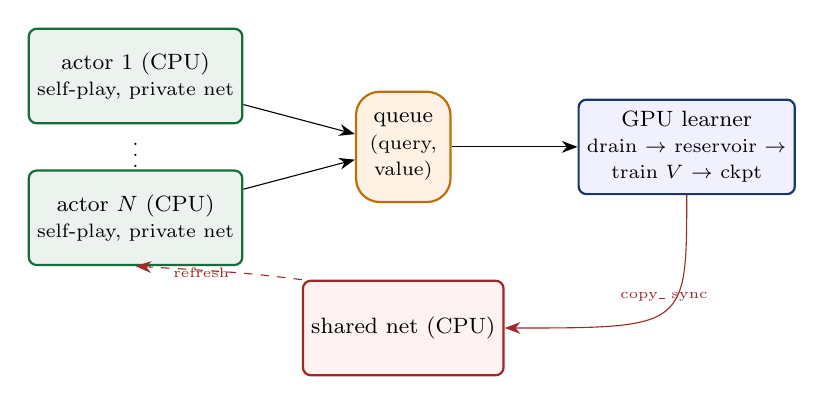
\begin{tikzpicture}[font=\footnotesize, >={Stealth[length=2mm]},
  a/.style={rectangle, rounded corners=1mm, draw=heroG, fill=heroG!8, thick,
            align=center, inner sep=3pt, minimum height=12mm},
  l/.style={rectangle, rounded corners=1mm, draw=accent, fill=blue!6, thick,
            align=center, inner sep=3pt, minimum height=12mm},
  q/.style={rectangle, rounded corners=3mm, draw=memO, fill=orange!10, thick,
            align=center, minimum height=14mm, minimum width=12mm, inner sep=2pt}]
  \node[a] (a1) at (0,0.9) {actor 1 (CPU)\\ \scriptsize self-play, private net};
  \node[a] (a2) at (0,-0.9){actor $N$ (CPU)\\ \scriptsize self-play, private net};
  \node[font=\scriptsize] at (0,0) {$\vdots$};
  \node[q] (qu) at (3.4,0) {queue\\ \scriptsize (query,\\ \scriptsize value)};
  \node[l] (le) at (7.0,0) {GPU learner\\ \scriptsize drain $\to$ reservoir $\to$\\ \scriptsize train $V$ $\to$ ckpt};
  \node[a, draw=villR, fill=red!5] (sh) at (3.4,-2.3) {shared net (CPU)};
  \draw[->] (a1) -- (qu); \draw[->] (a2) -- (qu); \draw[->] (qu) -- (le);
  \draw[->, villR] (le.south) .. controls (7,-2.3) .. node[above,font=\tiny]{copy\_ sync} (sh.east);
  \draw[->, villR, dashed] (sh.north west) .. controls (1.4,-1.6) .. node[left,font=\tiny]{refresh}(a2.south);
\end{tikzpicture}
\end{center}

Three bring-up gotchas, each a real bug and each documented in code: actors
forward through a \textbf{private} net refreshed only \emph{between} games (never
read a tensor the learner is mid-\texttt{copy\_}); \textbf{BLAS pinned to one
thread} before NumPy loads (a multithreaded OpenBLAS pool does not survive
process spawn); and a \textbf{watchdog respawns} dead actors. Checkpoints save the
state dict plus a TorchScript trace for a future C++/FFI consumer.

% ════════════════════════════════════════════════════════════════════════════
\section{Correspondence at a glance, and what is validated}
% ════════════════════════════════════════════════════════════════════════════

\begin{center}\small
\begin{tabular}{@{}lll@{}}
\toprule
ReBeL idea (tutorial) & file & key symbol \\
\midrule
public belief state                       & \file{pbs.py}            & \fn{PublicState}, \fn{encode\_query} \\
depth-limited subgame (shape only)        & \file{public\_tree.py}   & \fn{build\_*\_subgame}, \fn{subtree\_subgame} \\
chance node / Bayes over board cards      & \file{public\_tree.py}   & \fn{Node.is\_chance}, \fn{\_sample\_chance} \\
CFR inside the subgame, leaves co-evolve  & \file{subgame\_solver.py}& \fn{CfrSolver.step} \\
leaf $=$ net output $\times$ opp mass     & \file{subgame\_solver.py}& \fn{\_compute\_net\_leaf\_values} \\
value net $V(\text{PBS})$                 & \file{models.py}         & \fn{ValueNet}, \fn{NetValueFn} \\
self-play episode (6 steps)               & \file{recursive.py}      & \fn{RlRunner.step} \\
play a random CFR iterate (safety)        & \file{recursive.py}      & \texttt{act\_iter} split \\
value target $=$ root values of $\bar\sigma$& \file{subgame\_solver.py}& \fn{get\_hand\_values} \\
exploitability (the gate)                 & \file{exploitability.py} & \fn{exploitability\_bb} \\
training loop / reservoir                 & \file{train.py}, \file{replay.py} & \fn{train}, \fn{QueryValueBuffer} \\
scale (rank/incidence leaves)             & \file{showdown.py}       & \fn{RiverShowdown}, \fn{FoldRemoval} \\
cluster (actors $+$ learner)              & \file{rebel\_mp\_gpu.py} & \fn{\_actor\_loop}, \fn{main} \\
\bottomrule
\end{tabular}
\end{center}

\paragraph{Validation (every layer has a hard gate).}
\begin{itemize}[leftmargin=1.4em, itemsep=0pt]
\item \textbf{Solver vs ground truth}: river endgames solve to $\sim\!2\times10^{-4}$
  bb/hand; 10\,bb push/fold reproduces the Nash oracle (SB-jam/BB-call ranges
  agree $\sim$99\%, $\sim$3.6\,mbb/hand exploitable).
\item \textbf{Chance node}: full turn$\to$river ground truth solves to 0.027
  bb/hand; the all-in runout equity matches an independent \texttt{evaluate7}
  tally over the 44 valid river cards.
\item \textbf{Value-net mechanism}: self-play drives the recursive strategy's
  exploitability $2.0\to0.04$ (river) and $0.25\to0.03$ (turn$\to$river).
\item \textbf{Scaling}: rank/incidence leaves match the dense matrices to
  $10^{-11}$ for all hands; exploitability byte-identical.
\end{itemize}

\vfill
\begin{center}\small\itshape
The code is the source of truth; this document is a reading guide. Where a claim
here and the code disagree, the code (and its tests) win.
\end{center}

\end{document}
